\documentclass{article}
\usepackage[letterpaper, margin=1in]{geometry}
\usepackage{pgfplots}

\setlength{\parindent}{0pt}
\pgfplotsset{compat=1.18}

\title{Resource Math}
\author{Justin Ottesen}
\date{Last Modified: \today}

\begin{document}

  \maketitle

  This information is consistent with release 1.3.1

  \section*{Chips}

  Chips are the simple money of the game. They are only produced by money towers. One is guaranteed at the start of the game, the other way players can create them is by finding ruins and using 24 paint (more on paint later) to make a special pattern, and spending chips. The table below shows the cost of creating / upgrading money towers:
  \begin{center}
    \begin{tabular}{c | c | c}
      Level & Upgrade Cost (Chips) & Mining Rate (Chips / Turn) \\
      \hline 
      1 & 1000 & 20   \\
      2 & 2500 & 30   \\
      3 & 5000 & 40   \\
    \end{tabular}
  \end{center}
  This is also summarized in the graph below:
  \begin{center}
    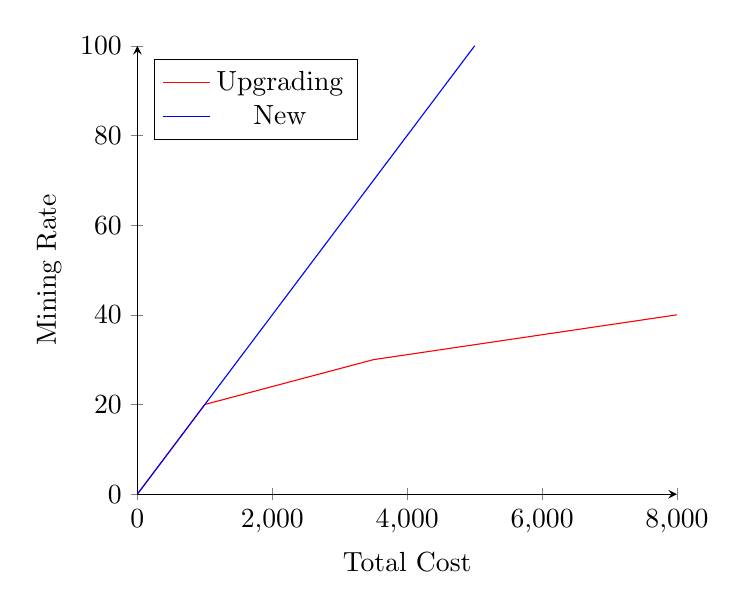
\begin{tikzpicture}
      \begin{axis}[
        axis lines = left,
        xlabel = Total Cost,
        ylabel = Mining Rate,
        legend pos = north west
      ]
      \addplot [
        color = red
      ]
      coordinates {
        (0,0)(1000,20)(3500,30)(8000,40)
      };
      \addlegendentry{Upgrading}

      \addplot [
        color = blue,
        domain = 0:5000
      ]
      { x / 50 };
      \addlegendentry{New}
        
      \end{axis}
    \end{tikzpicture}
  \end{center}
  This makes it pretty clear that while building new Money Towers is an option (there are still available runes), this is the most cost-effective choice. Since each level 1 tower produces 20 chips per turn, a new tower should pay for itself in 500 turns.

  \section*{Paint}

  Paint is a per-unit resource. Moppers can transfer paint to both robots and towers, robots must take paint from the towers. Paint can be collected in two ways:
  \begin{enumerate}
    \item \textbf{Paint Towers:} Paint towers passively collect paint each turn.
    \item \textbf{Moppers:} Moppers receive 5 paint when they mop a square that an enemy is on.
  \end{enumerate}
  Paint towers are the more reliable way of getting this resource, since presumably enemy robots will avoid moppers if they are smart. Any mopper income will be considered a bonus.

  \medskip

  Each team starts with one Paint Tower, and can build more at ruins. Paint Towers can be upgraded to produce paint more quickly. Initially, each tower will produce 5 paint per round, increasing by 5 with every level. The table of costs and paint generation is shown below:
  \begin{center}
    \begin{tabular}{c | c | c}
      Level & Upgrade Cost (Chips) & Mining Rate \\
      \hline 
      1 & 1000 & 5    \\
      2 & 2500 & 10   \\
      3 & 5000 & 15   \\
    \end{tabular}
  \end{center}
  We can show this information in the chart below as well:
  \begin{center}
    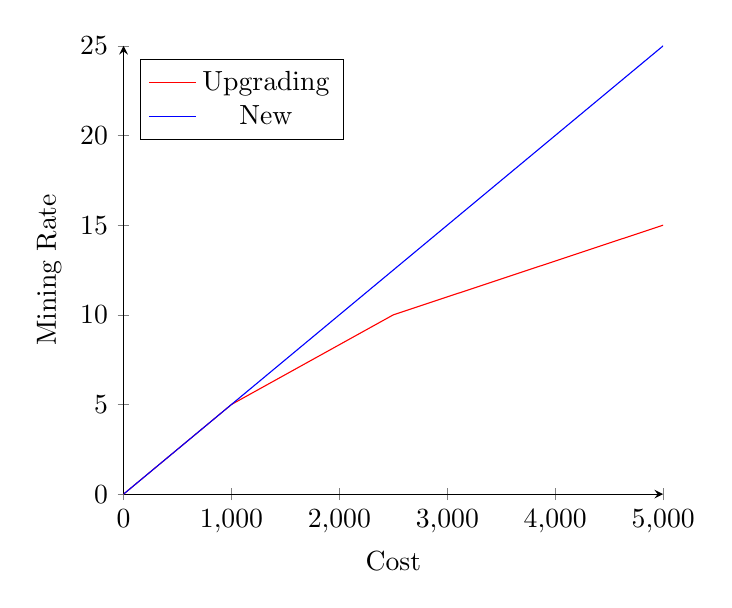
\begin{tikzpicture}
      \begin{axis}[
        axis lines = left,
        xlabel = Cost,
        ylabel = Mining Rate,
        legend pos = north west
      ]
      \addplot [
        color = red
      ]
      coordinates {
        (0,0)(1000,5)(2500,10)(5000,15)
      };
      \addlegendentry{Upgrading}

      \addplot [
        color = blue,
        domain = 0:5000
      ]
      { x / 200 };
      \addlegendentry{New}
        
      \end{axis}
    \end{tikzpicture}
  \end{center}
  Again, building new towers is clearly the better deal in terms of chips. Another important note, \textbf{each tower starts with 500 paint}, which is another huge reason to favor creating new towers over upgrading existing ones.

  \section*{Special Resource Patterns}

  Towers can also be boosted using Special Resource Patterns (SRPs). When painted on the ground, they will boost the resource collection rate of all towers by 3 units per turn. To create a new tower, 24 paint and 1,000 chips must be used. 

  \medskip

  Because new towers have such a large paint reward, the limiting resource will likely be chips. Special resource patterns should be created wherever painting occurs, but towers should be prioritized.

  \begin{center}
    LOOK MORE INTO THIS
  \end{center}

  \section*{Disintegration}

  \begin{center}
    LOOK MORE INTO THIS, TRADE 1000 CHIPS FOR 500 PAINT
  \end{center}

  \section*{Robots}

  The following table shows the costs of creating different robot types:

  \begin{center}
    \begin{tabular}{c | c | c}
      Type & Chips & Paint \\
      \hline
      Soldier & 250 & 200 \\
      Splasher & 400 & 300 \\
      Mopper & 300 & 100
    \end{tabular}
  \end{center}

  Note that the paint costs aren't necessarily "costs", since the paint goes directly to the created robot's inventory.

  \section*{Applications}

  \subsection*{Early Game}
  Each player starts with two towers, one Paint Tower and one Money Tower. Each of these has 500 paint and a total of 1,000 chips to share. This also means that the resource generation rate is 20 chips and 5 paint per turn.

  \medskip

  Each tower ($2 \times$) should create one soldier (200 paint, 250 chips) and one mopper (100 paint, 300 chips) for a total cost of 600 paint and 1100 chips. One of these towers will need to wait until round 6 to produce its mopper in order to accumulate the 100 extra chips.

  \medskip

  One soldier and one mopper is the minimum "safe" start for robots. The soldier will be doing the painting, and the mopper will clear enemy painted tiles. The splasher could be considered as an alternative to the soldier, but at a cost of 400 chips it is far too expensive, and would delay the first mopper to round 6 and second to round 26. If the devs change the initial conditions, this can be revisited.

  \medskip

  The first priority should be finding and painting new ruins to boost chip production. It will take until round 56 to produce the first new tower assuming no resource patterns (which would decrease the time) or other robots (which would increase the time) are created.

  \medskip

  The big challenge will be defending this area. Since we need to save until round 56 to build the tower, this means the opponent has 2120 chips to stop us from doing so, which is more than enough to overwhelm a single soldier and mopper.

  \subsection*{Main Game}

  Chip management will be the economic focus of the main game. We should be prepared to build 

  \subsection*{Win Conditions \& Endgame}

  The main win condition is 70\% coverage of the paintable squares on the map. Since the map is between $20 \times 20$ and $60 \times 60$ (inclusive), that means that (an upper bound estimate of) the number of painted tiles necessary to win is \verb|(width * height) * 0.7|. For a $20 \times 20$ grid, this is 280 squares, and for $60 \times 60$ this is 2520. If the maximum number of walls is used (20\% of the map), these numbers drop to 224 and 2016. On a small map, it is entirely possible win within 200 rounds.
  \begin{center}
    SMALLER MAPS BETTER TO STOP TOWERS EARLY AND SPAM SOLDIERS?
    
    DO THE MATH AND CHECK. SMALLER ALSO MEANS OPPONENT IS CLOSER, SO WILL LIKELY HAVE COMBAT EARLIER.
  \end{center}


\end{document}